\chapter{Filters and System Efficiency}

\begin{table}
\centering
\caption{Filters}
\medskip
\label{table:filters}
\footnotesize
\begin{tabular}{lcccccl}
\toprule
Filter&$\lambda_\mathrm{S}$&$\lambda_\mathrm{L}$&$\Delta\lambda$&$\bar\eta$&$n_0$&\multicolumn{1}{c}{Color Term}\\
&nm&nm&nm&&\unit{e/s}\\
\midrule
\multicolumn{7}{c}{Blue Channel}\\
\midrule
$B$   & 386.6 & 486.3 & \phantom{}101.4 & 0.32 & $2.5 \times 10^{9\phantom{0}}$ & $+0.24 \times (B-V)$\\
$g$   & 397.0 & 549.1 & \phantom{}152.2 & 0.40 & $5.3 \times 10^{9\phantom{0}}$ & $-0.05 \times (g-r)$\\
$r$   & 553.5 & 694.7 & \phantom{}141.3 & 0.40 & $5.0 \times 10^{9\phantom{0}}$ & $+0.00 \times (g-r)$\\
$i$   & 690.4 & 812.1 & \phantom{}121.7 & 0.39 & $3.4 \times 10^{9\phantom{0}}$ & $-0.04 \times (g-r)$\\
$gri$ & 399.1 & 811.6 & \phantom{}412.8 & 0.39 & $1.3 \times 10^{10\phantom{}}$ & $-0.07 \times (g-r)$\\
\midrule
\multicolumn{7}{c}{Red Channel}\\
\midrule
$z$   & 825.9 & 915.1 & \phantom{0}89.6 & 0.33 & $1.5 \times 10^{9\phantom{0}}$ & $+0.01 \times (r-i)$\\
$y$   & 917.8 & 972.8 & \phantom{0}57.4 & 0.26 & $7.4 \times 10^{8\phantom{0}}$\\
$zy$  & 826.7 & 939.7 & \phantom{}125.2 & 0.35 & $2.2 \times 10^{9\phantom{0}}$ & $+0.09 \times (r-i)$\\
\bottomrule
\end{tabular}
\end{table}


\section{Filters}

The DDRAGO filters are summarized in Table~\ref{table:filters}.

The blue channel has $g$, $r$, and $i$ filters that are very similar to the corresponding Pan-STARRS filters, a wide $gri$ filter that passes from the blue edge of $g$ to the red edge of $i$ and is very similar to the Pan-STARRS $w$ filter, and a $B$ filter. (It can be somewhat confusing that the blue channel has red $r$ and infrared $i$ filters, but it's too late to change this established usage.)

The red channel has $z$ and $y$ filters that are very similar to the corresponding Pan-STARRS filters and a wide $zy$ filter that passes from the blue edge of $z$ and thus is similar to SDSS $z$.

The $g$, $r$, $i$, $z$, $y$, $gri$, and $zy$ filters are interference filters on fused silica substrates. The $B$ filter is a conventional cemented assembly of colored glasses.

The DDRAGO $i$ and $z$ filters were deliberately designed to be slightly different from their Pan-STARRS equivalents \citep{Tonry-2012}. The Pan-STARRS $i$ and $z$ filters overlap slightly and cross at about 818~nm. The DDRAGO $i$ and $z$ filters are separated, with the $i$ filter having its half-maximum at 812~nm and the $r$ filter at 825~nm. This is so that the bandpasses are largely defined by the filters and not by the D2 transition from reflectance to transmittance, which depends on polarization. This is especially important in DDRAGO, since there are reflections from inclined surfaces at M3, D1, and D2, and these rotate as the telescope tracks a field. The same considerations apply to the $gri$ and $zy$ filters. These separations can most clearly be seen in Figures~\ref{figure:system-filters-grizy} and \ref{figure:system-filters-others}.


\section{Transformations}

Table~\ref{table:filters} shows typical color terms for the transformations from natural magnitudes to the corresponding magnitudes in the Pan-STARRS and Landolt systems. We transform $gri$ to Pan-STARRS $r$, not to Pan-STARRS $w$. The color terms are in the sense
\begin{align}
\mbox{Standard magnitude} = \mbox{DDRAGO magnitude} + \mbox{color term}.
\end{align}
For most filters, the color terms are small. The exception is $B$, for which the color term is $+0.24(B-V)$.

\section{System Efficiency}

We have modeled the system efficiency of the instrument at 1.5 airmasses, taking into account:
\begin{itemize}
\item The continuum absorption 300 nm to 2000 nm calculated using the “k-model” from \cite{Schuster-2001}, without ozone, and extrapolated from the last data point using their assumed RC index of $-4.05$ and derived aerosol index of $-0.87$. 

\item
The atmospheric line-absorption spectrum above 850~nm generated using ATRAN (Lord 1992), made available on the SOFIA web site by Dr.\ William Vacca. The altitude was specified as 2790 meters and, following advice on the web page, the latitude was left at the default of 39 degrees. We assume an airmass of 1.5 and a water vapor burden of 2.8~mm (the median value given by \cite{Otarola-2009}. The lower wavelength limit of 0.85 µm is a limitation of ATRAN. It means that the absorption-line spectrum does not contain absorption from either the strong A-band (760 to 763~nm) and B-band (686 to 689~nm) or from other weaker lines.

\item
Three reflections from aluminium. We use the measurement reported by \cite{Boccas-2006} for a \emph{fresh} aluminum coating at Gemini.  As the mirrors age, the reflectivity will decrease.

\item
Models of the transmissions of L1, L2, L3, and L4, including anti-reflection coatings and internal absorption.

\item
Vendor-supplied transmission and reflectance measurements for D1, D2, and the filters.

\item
Vendor-supplied transmission date for the CCD windows and quantum efficiency data for the CCDs.

\end{itemize}

\begin{figure}
\centering
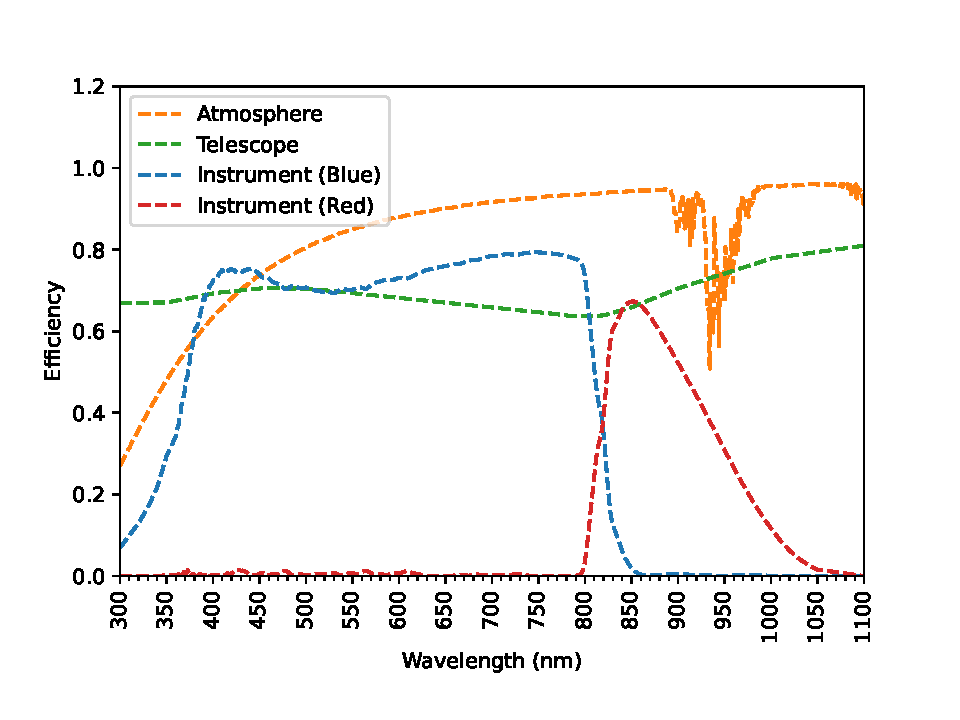
\includegraphics[width=0.80\linewidth]{figure/components.pdf}
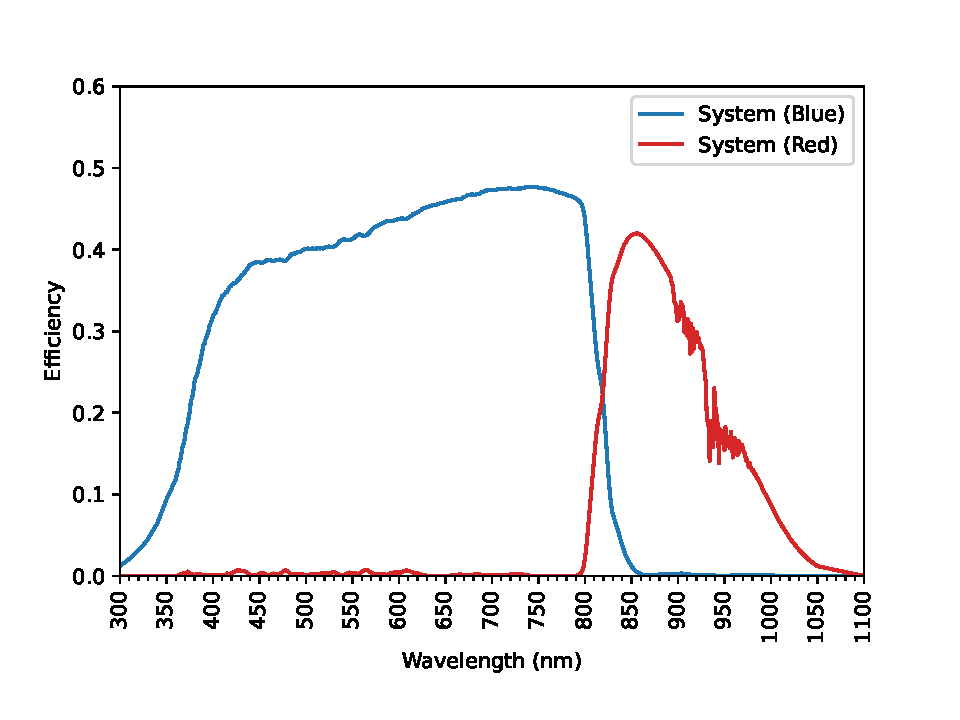
\includegraphics[width=0.80\linewidth]{figure/system.pdf}
\caption{Top: The major components of the system efficiency at 1.5 airmasses: the atmosphere, telescope, and the efficiencies of the blue and red channels of the instrument without filters. Bottom: The system efficiencies of the blue and red channels without filters.}
\label{figure:system-efficiency}
\end{figure}

\begin{figure}
\centering
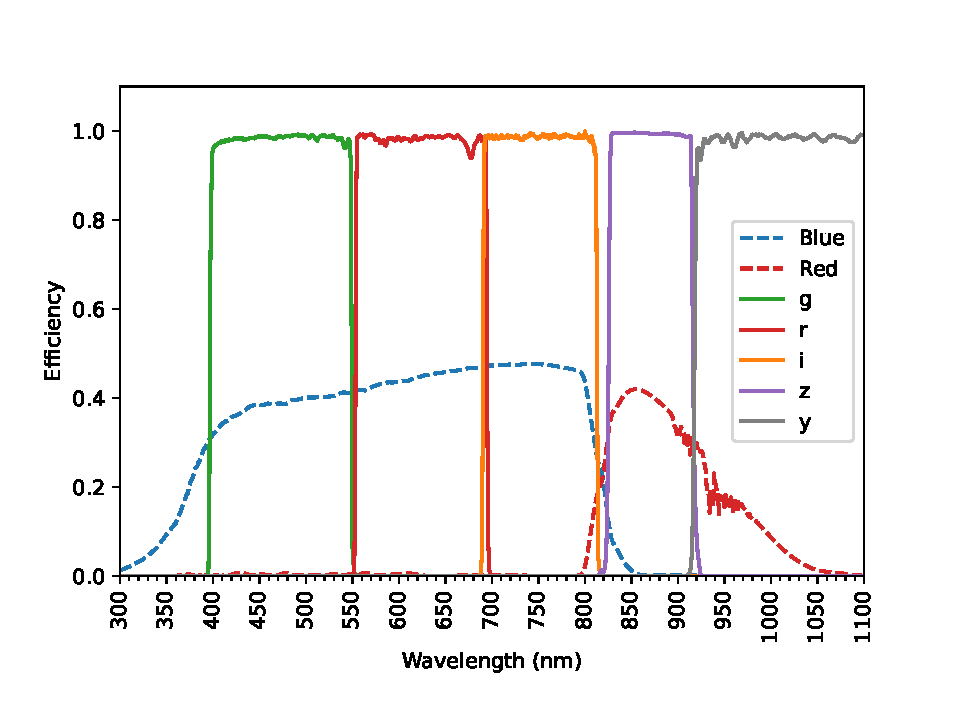
\includegraphics[width=0.80\linewidth]{figure/filters-0.pdf}
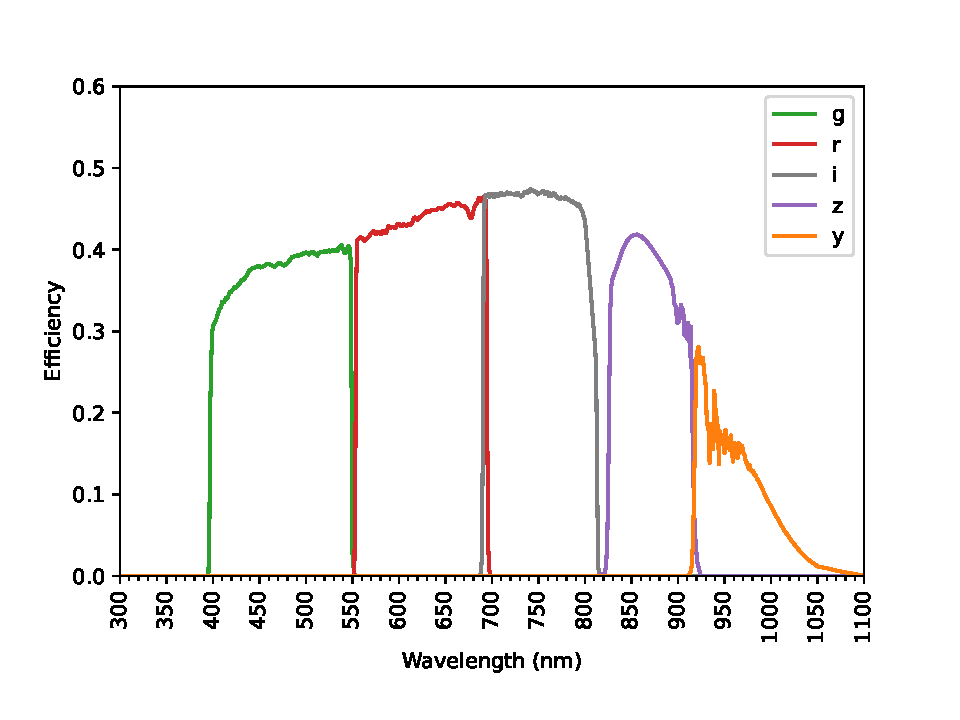
\includegraphics[width=0.80\linewidth]{figure/system-filters-0.pdf}
\caption{Top: the transmission of the $g$, $r$, $i$, $z$, and $y$ filters and the system efficiencies of the blue and red channels without filters. Bottom: the system efficiencies including the $g$, $r$, $i$, $z$, and $y$ filters. Note that the D2 dichroic encroaches on the red edge of the $i$ filter and the blue edge of the $z$ filter.}
\label{figure:system-filters-grizy}
\end{figure}

\begin{figure}
\centering
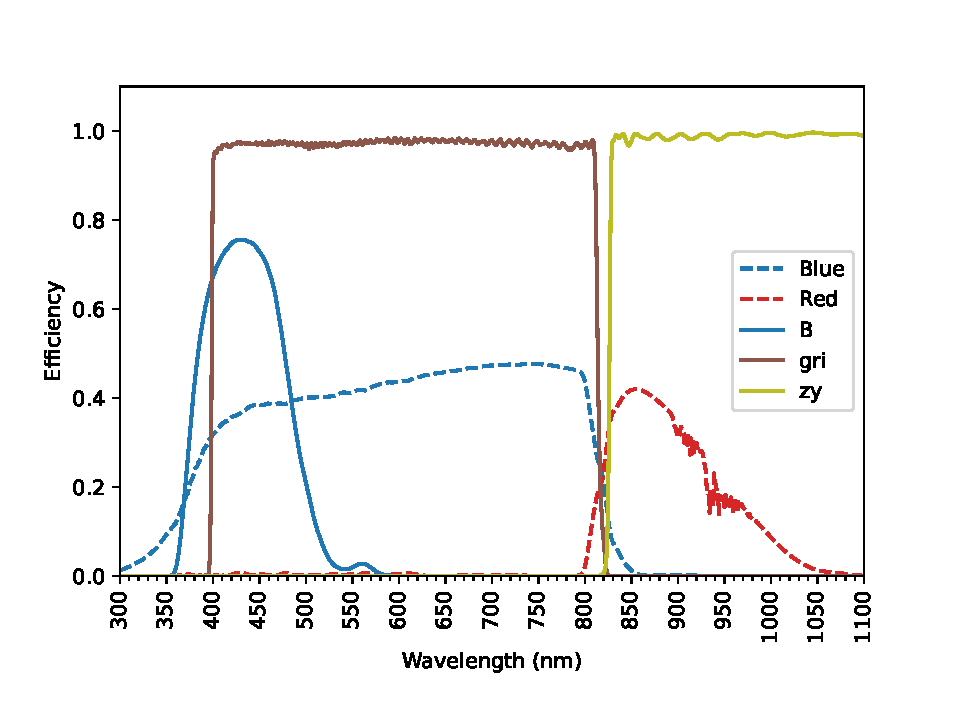
\includegraphics[width=0.80\linewidth]{figure/filters-1.pdf}
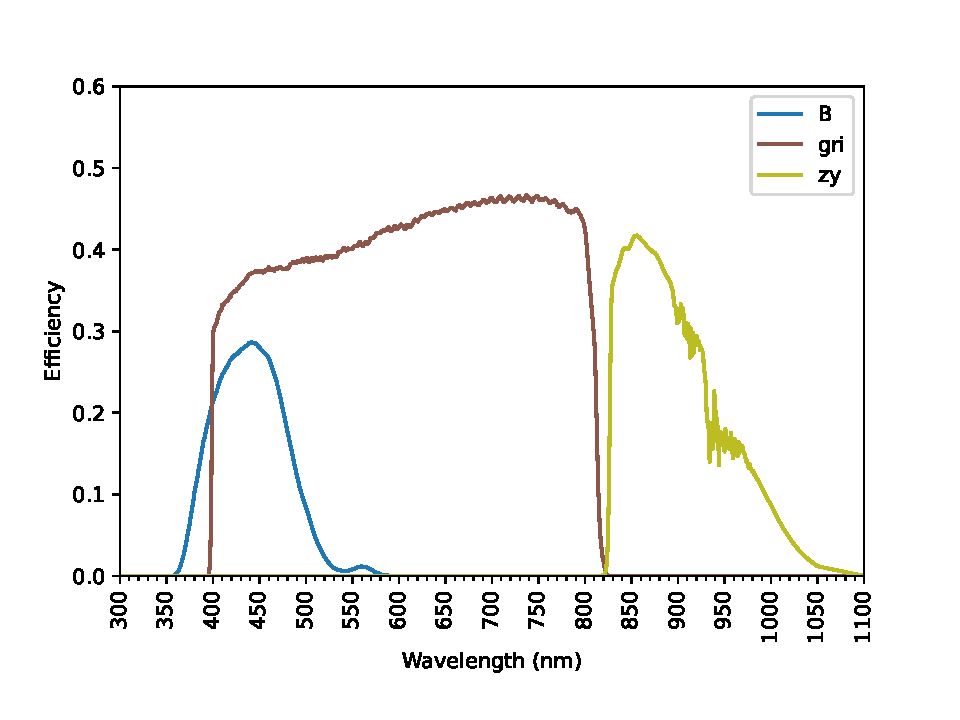
\includegraphics[width=0.80\linewidth]{figure/system-filters-1.pdf}
\caption{Top: the transmission of the $B$, $gri$, and $zy$ filters and the system efficiencies of the blue and red channels without filters. Bottom: the system efficiencies including the $B$, $gri$, and $zy$ filters. Note that the D2 dichroic encroaches on the red edge of the $gri$ filter and the blue edge of the $zy$ filter.}
\label{figure:system-filters-others}
\end{figure}

\begin{figure}
\centering
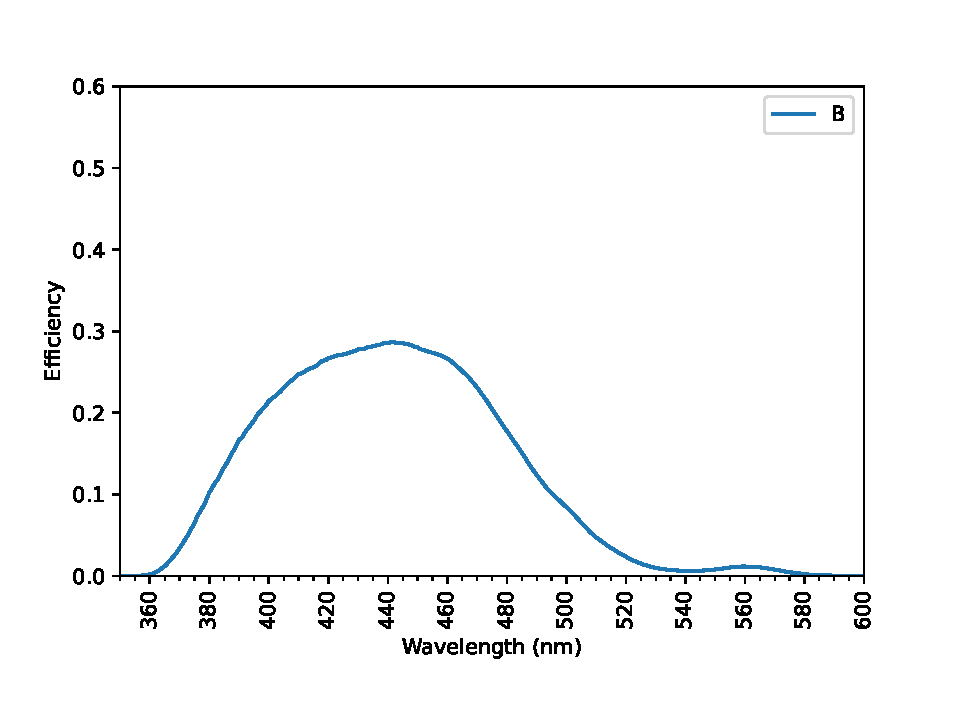
\includegraphics[width=0.80\linewidth]{figure/system-B.pdf}
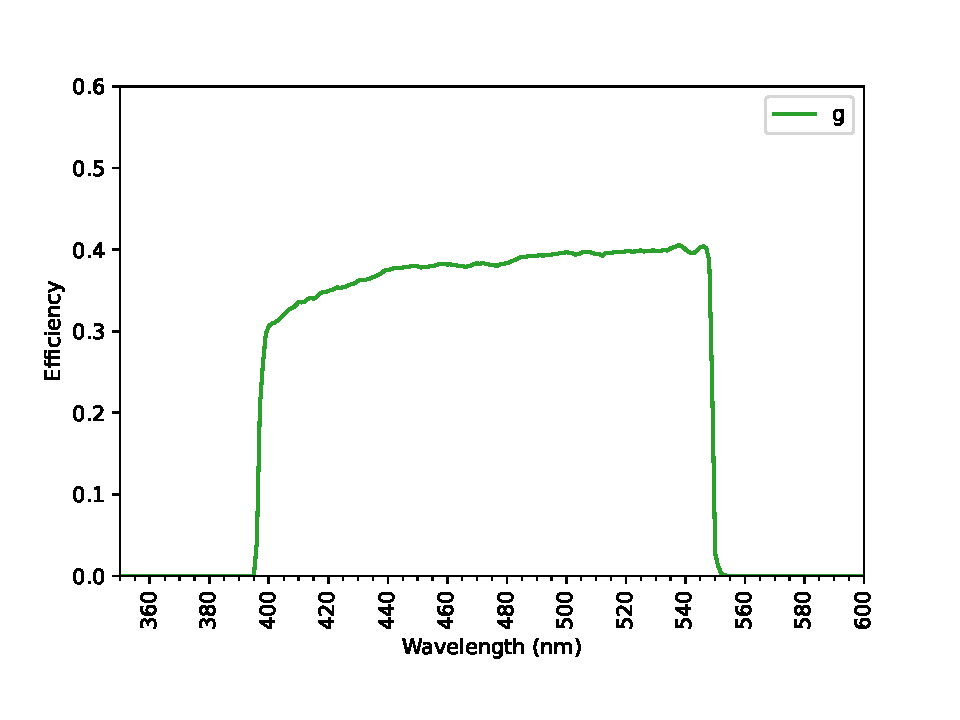
\includegraphics[width=0.80\linewidth]{figure/system-g.pdf}
\caption{The system efficiencies in the $B$ and $g$ filters.}
\label{figure:system-filters-first}
\end{figure}

\begin{figure}
\centering
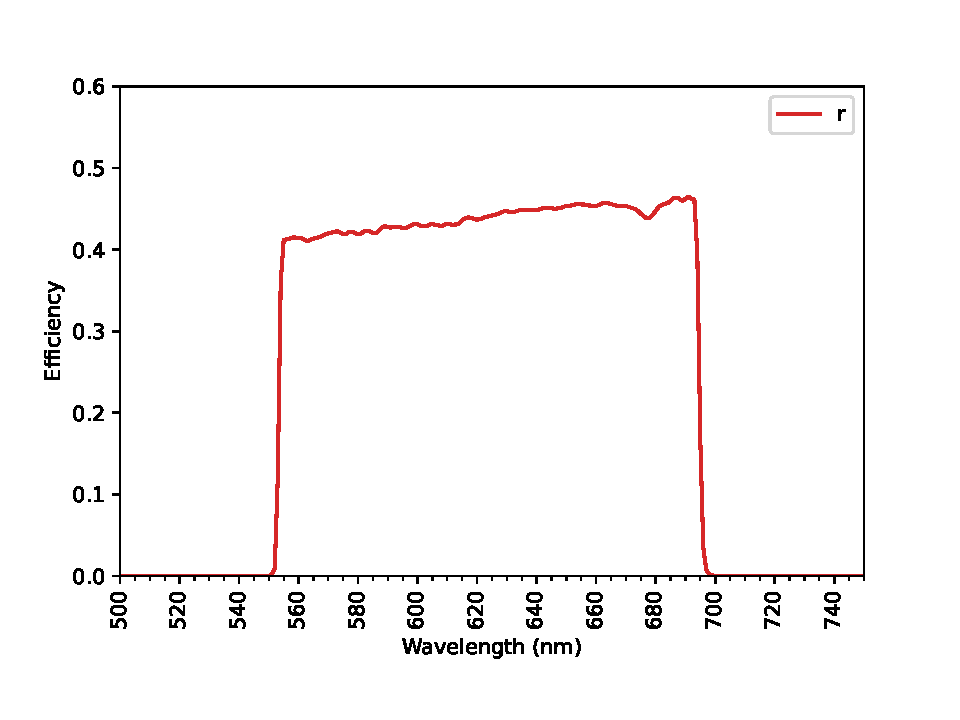
\includegraphics[width=0.80\linewidth]{figure/system-r.pdf}
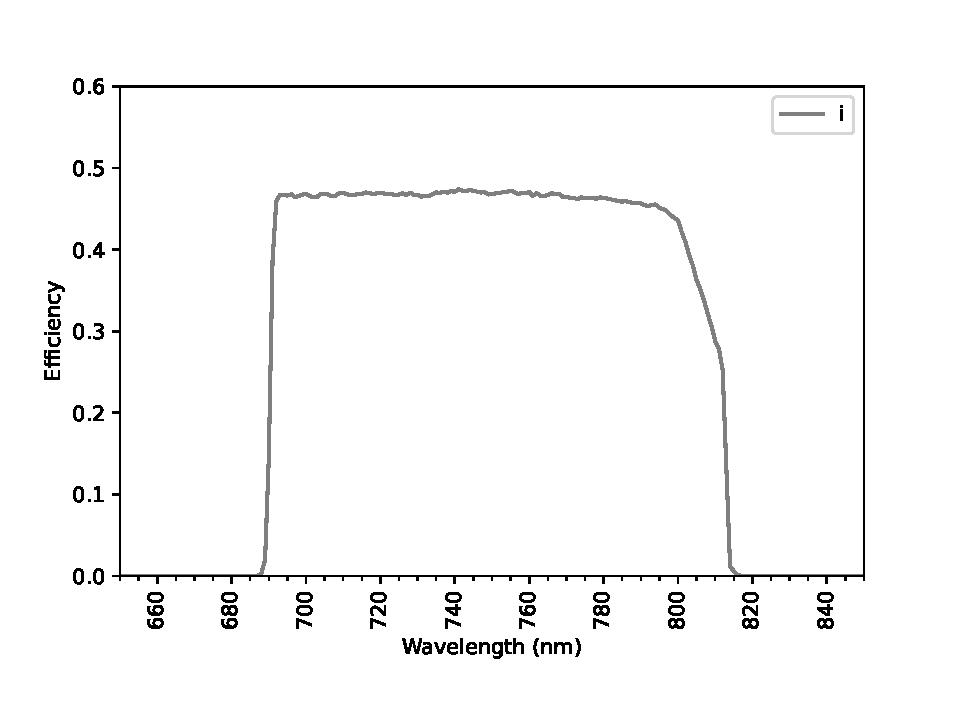
\includegraphics[width=0.80\linewidth]{figure/system-i.pdf}
\caption{The system efficiencies in the $r$ and $i$ filters.}
\end{figure}

\begin{figure}
\centering
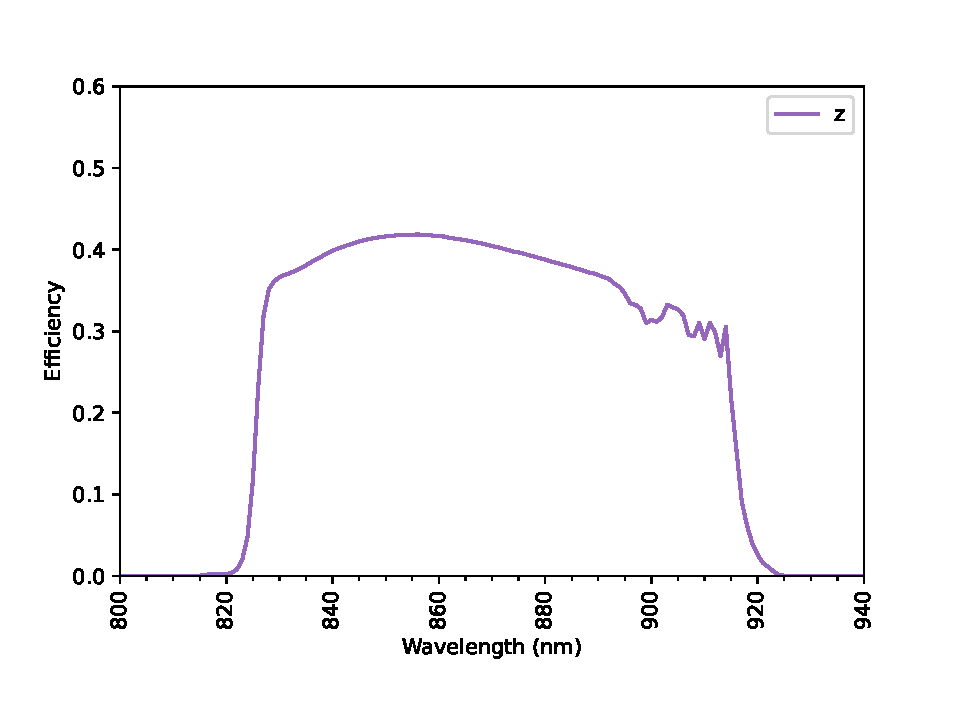
\includegraphics[width=0.80\linewidth]{figure/system-z.pdf}
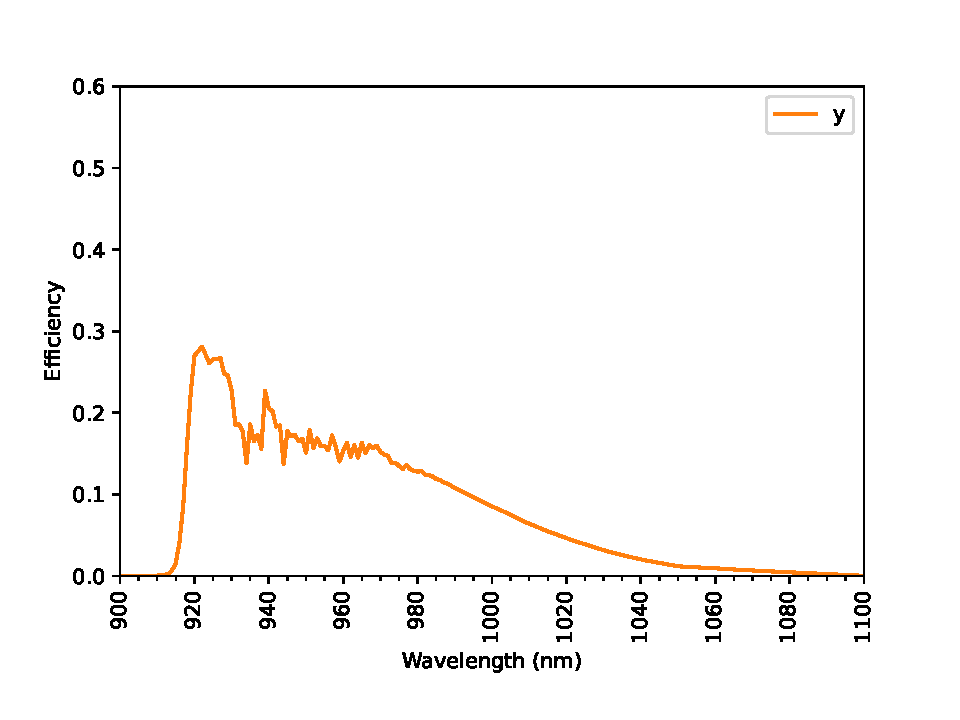
\includegraphics[width=0.80\linewidth]{figure/system-y.pdf}
\caption{The system efficiencies in the $z$ and $y$ filters.}
\end{figure}


\begin{figure}
\centering
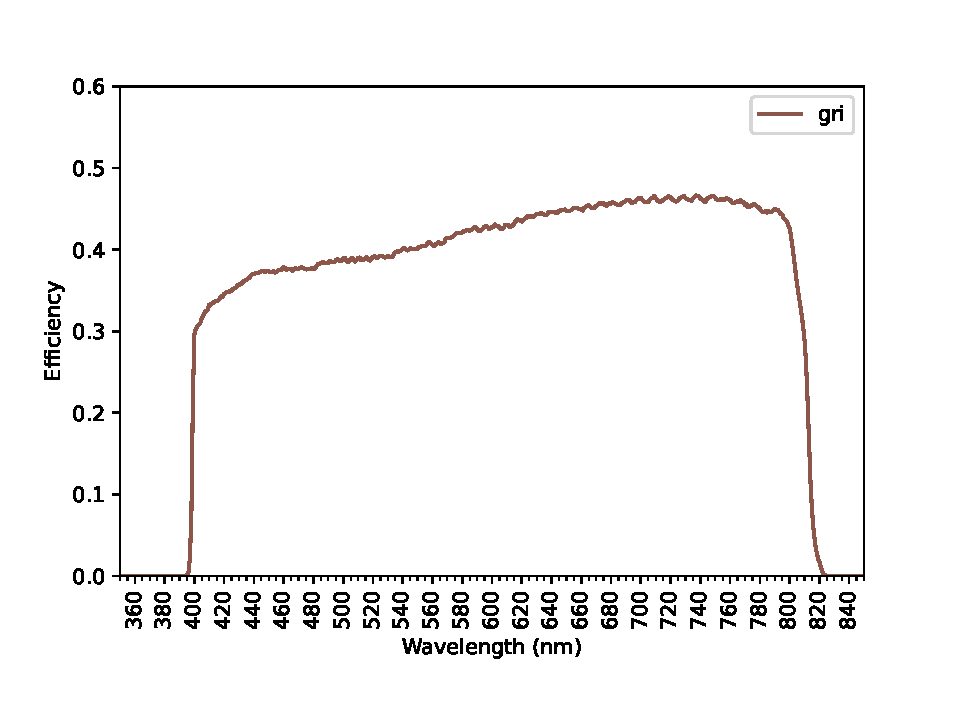
\includegraphics[width=0.80\linewidth]{figure/system-gri.pdf}
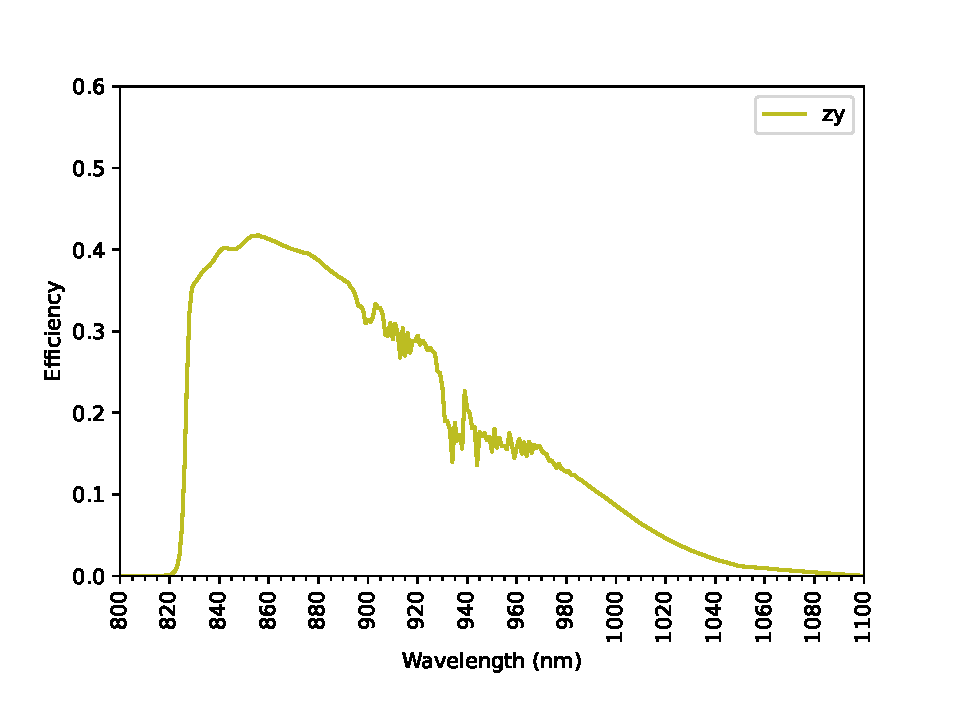
\includegraphics[width=0.80\linewidth]{figure/system-zy.pdf}
\caption{The system efficiencies in the $gri$ and $zy$ filters.}
\label{figure:system-filters-last}
\end{figure}

Figure~\ref{figure:system-efficiency} shows the major components of the total system efficiency without filters --- the atmosphere, the telescope, and the efficiencies of the blue and red channels including both optics and the detector --- and the total system efficiencies in the blue and red channels.

Figures~\ref{figure:system-filters-grizy} and \ref{figure:system-filters-others} show the transmission of the filters alone and the system efficiency including the filters. They show how the dichroic transition in D2 modifies slightly the red edges of the $i$ and $gri$ filters and the blue edges of the $z$ and $zy$ filters and how the detector fall-off modifiers significantly the response in the $z$, $y$, and $zy$ filters.

Figures~\ref{figure:system-filters-first} and \ref{figure:system-filters-last} show in detail the total system efficiency $\eta$ for each filter. Table~\ref{table:filters} gives the full-width-at-half-maximum $\Delta\lambda$ and the short and long half-maximum wavelengths $\lambda_\mathrm{S}$ and $\lambda_\mathrm{L}$ for the total system efficiency. It also gives the mean efficiency $\bar\eta$, defined by
\begin{align}
\bar\eta \Delta\lambda \equiv \int \eta\,d\lambda.
\end{align}
The mean efficiency would be the efficiency of a rectangular filter with width $\Delta\lambda$ and with the same integrated efficiency $\int \eta\,d\lambda$ as the real filter.

\section{Zero-Points}

Table~\ref{table:filters} also gives the estimated zero points $n_0$ for each filter, defined by 
\begin{align}
n_0 = \frac{A F_0}{h}\int \frac{\eta}{\lambda}\,d\lambda,
\end{align}
in which $A$ is the area of the telescope (discounting the central obstruction), $h$ is Planck's constant, and $F_0 = 3631~\unit{Jy}$ is the flux density of a source with $\AB = 0$. In practical terms, the zero point $n_0$ is the expected signal in $\unit{e/s}$ from a source with zero AB magnitude at all wavelengths.

Observers are cautioned that these zero points are optimistic, in that they assume fresh aluminum coatings. The M1 and M2 mirrors were coated in June and September 2024, and the reflectivity is expected to decrease by about 10\% per year. Furthermore, clouds can also reduce the observed signal.

NOTE: We are still working to confirm the measured zero points, but at the moment there is no reason to believe that the theoretical estimates are significantly incorrect.
